\documentclass[11pt, a4paper]{article}
\usepackage{graphicx, fullpage, hyperref, listings}
\usepackage{appendix, pdfpages, color}
\usepackage{indentfirst} %段首空两格 棒
\usepackage{chngpage} 
\usepackage{tocloft}            % This squashes the Table of Contents a bit
\usepackage{pdfpages}
\usepackage{multirow}
\usepackage{amsmath}
\usepackage{amssymb}
\usepackage{framed}

%% Used on windows
%\usepackage[UTF8]{ctex}
%\usepackage{array}%需要该宏包

%% Used On Ubuntu
\usepackage{CJKutf8}


\setlength\cftbeforesecskip{3pt}
\renewcommand{\contentsname}{\centerline{\textbf{Content}}}
\graphicspath{{images/}}

\usepackage{multicol}

\usepackage{graphicx}
\usepackage{epstopdf}
\hypersetup{CJKbookmarks,%
	bookmarksnumbered,%
	colorlinks,%
	linkcolor=black,%
	citecolor=black,%
	plainpages=false,%
	pdfstartview=FitH}

%%%%%%%代码语法高亮设置

\usepackage{color}

\definecolor{pblue}{rgb}{0.13,0.13,1}
\definecolor{pgreen}{rgb}{0,0.5,0}
\definecolor{pred}{rgb}{0.9,0,0}
\definecolor{pgrey}{rgb}{0.46,0.45,0.48}

\usepackage{listings}
\lstset{
	language=Java,
	showspaces=false,
	showtabs=false,
	%%%%%
	frame = single,
	stepnumber = 2,  
	numbersep = 4pt, 
	 numbers=left,
	%breakatwhitespace=false, 
	tabsize=2,  
	%%%%%
	breaklines=true,
	showstringspaces=false,
    breakatwhitespace=false, 
	commentstyle=\color{pgreen},
	keywordstyle=\color{pblue},
	stringstyle=\color{pred},
	basicstyle=\ttfamily,
	%moredelim=[il][\textcolor{pgrey}]{$$},
	%moredelim=[is][\textcolor{pgrey}]{\%\%}{\%\%},
}


%%%%%%%%代码语法高亮设置

\definecolor{MyLightYellow}{cmyk}{0,0.,0.2,0} 

\setlength{\parskip}{4pt}        % sets spacing between paragraphs
\interfootnotelinepenalty=500    % this prevents footnotes breaking across pages


\title{
\includegraphics[width=0.45\textwidth]{dg}
        \\AffectNet Paper Summary and Training Result  }          % <<<<<<<<< change the title as appropriate
\author{Jiaming Nie}                    % <<<<<<<<< module code

\begin{document}
\begin{titlepage}
	
%\date{\today}
\maketitle
\addtocontents{toc}{\protect\thispagestyle{empty}}
% because we don't want a page number on the title page
% Thanks to Huang Shanyue for suggesting this 

%\date{\today}
\thispagestyle{empty}  %去除首页页码
%\tableofcontents

\end{titlepage}

%\tableofcontents
%\listoffigures

%\newpage


\begin{CJK}{UTF8}{gbsn}
	
\section{AffectNet Paper 模型}

AffectNet的原paper利用了三种模型对人脸表进行进行建模分类,具体是三种:

\begin{table}[htbp] 
	\begin{center}
		\caption{AffectNet 中几种分类与回归模型}
		\begin{tabular}{|l|p{270pt}|} \hline
			Categorical Model & 分类模型,根据不同表情图片与标签进行分类   \\ \hline
			Dimensional Model & 纬度模型,基于不同表情的Arousal(情绪的强烈程度)和Valence(情绪的正负倾向),以上两个数值均为连续的。\\ \hline
			Facial Action Coding System (FACS) &  根据脸部提取的特征点,用于描述脸部表情的动作,并不直接给出表情的分类。 用Action Unit来表示。AU6和AU12可能均表示高兴。\\ \hline
		\end{tabular}
		
		\label{tab:kf_meaning}
	\end{center}
\end{table}

\section{模型Baseline}

\subsection{Categorical Model Baseline}

数据集本身并不均衡,对于不均衡的数据集,采取以下几种方式:

\begin{itemize}
\item Imbalanced learning
\item Down-Sampling 下采样
\item Up-Sampling 上采样
\item Weighted-Loss 加权损失
\end{itemize}

所用的CNN是AlexNet,并且数据在处理前,对图片进行256$/times$256的crop,并在数据增强阶段进行224$/times$224的random crop。

训练的参数:

\begin{itemize}
\item Epoch: 20
\item Batch Size: 256
\item Learning Rate: 0.01 (每隔10000次叠代下降10\%)
\item Momentum: 0.9
\end{itemize}

\subsubsection{不同模型下的结果}

如图\ref{Fig:t7}中所示,对于Original和skew-normalized下,top-1和top-2 F1 score的结果.

加权损失的表现是最好的.

\newpage

 \begin{figure}[htbp]
	
	\centering %使插入的图片居中显示
	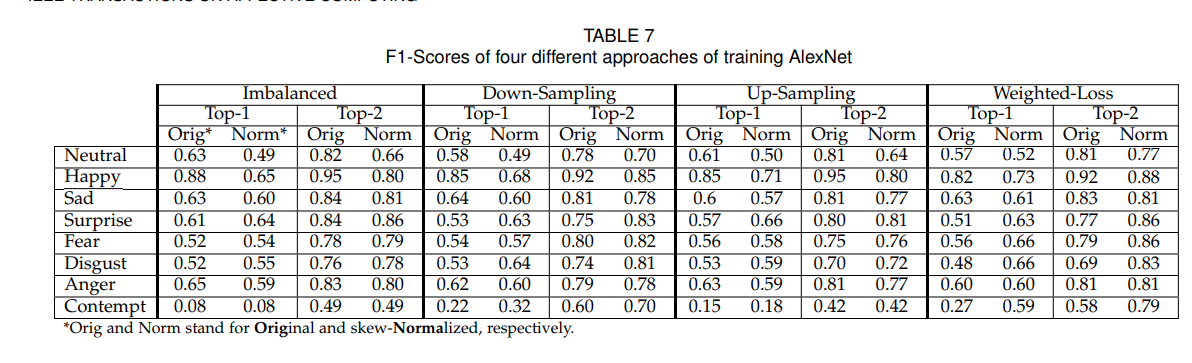
\includegraphics[width=10cm]{fscore}
	
	\caption{Top 2 F-score}
	\label{Fig:t7}
	%插入图片的标题,一般放在图片的下方,放在表格的上方
	
\end{figure}

\subsection{Dimensional Model Baseline}

\section{ResNet18 Training Result (Using Keras)}

	
	
	

\end{CJK}


%\tableofcontents

%\listoffigures
%\listoftables
%\lstlistoflistings        


%\newpage




\bibliographystyle{IEEEtran}  
%\bibliography{MyRefs} 
%\addcontentsline{toc}{section}{References}





%-------------------------------------------------------------------------------------------------------





\end{document}
